\documentclass{beamer}
%\documentclass[handout]{beamer}
%\usepackage[dvips]{color}
\usepackage{graphicx, hyperref}
\usepackage{amsmath,amssymb,array,comment,eucal}
\newcommand{\e}{\mathbf{e}}
\renewcommand{\P}{\mathbf{P}}
\newcommand{\F}{\mathbf{F}}
\newcommand{\R}{\textsf{R}}
\newcommand{\mat}[1] {\mathbf{#1}}
%\newcommand{\ind}{\mathrel{\mathop{\sim}\limits^{\mathit{ind}}}}
%\newcommand{\iid}{\mathrel{\mathop{\sim}\limits^{\mathit{iid}}}}
\newcommand{\E}{\textsf{E}}
\newcommand{\SE}{\textsf{SE}}
\newcommand{\SSE}{\textsf{SSE}}
\newcommand{\RSS}{\textsf{RSS}}
\newcommand{\FSS}{\textsf{FSS}}
\renewcommand{\SS}{\textsf{SS}}
\newcommand{\MSE}{\textsf{MSE}}
\newcommand{\SSR}{\textsf{SSR}}
\newcommand{\Be}{\textsf{Beta}}
\newcommand{\St}{\textsf{St}}
%\newcommand{\C}{\textsf{C}}
\newcommand{\GDP}{\textsf{GDP}}
\newcommand{\NcSt}{\textsf{NcSt}}
\newcommand{\Bin}{\textsf{Bin}}
\newcommand{\NB}{\textsf{NegBin}}
\renewcommand{\NG}{\textsf{NG}}
\newcommand{\N}{\textsf{N}}
\newcommand{\Ber}{\textsf{Ber}}
\newcommand{\Poi}{\text{Poi}}
\newcommand{\Gam}{\textsf{Gamma}}
\newcommand{\BB}{\textsf{BB}}
\newcommand{\Gm}{\textsf{G}}
\newcommand{\Un}{\textsf{Unif}}
\newcommand{\Ex}{\textsf{Exp}}
\newcommand{\DE}{\textsf{DE}}
\newcommand{\tr}{\textsf{tr}}
\newcommand{\cF}{{\cal{F}}}
\newcommand{\cL}{{\cal{L}}}
\newcommand{\cI}{{\cal{I}}}
\newcommand{\cB}{{\cal{B}}}
\newcommand{\cP}{{\cal{P}}}
\newcommand{\bbR}{\mathbb{R}}
\newcommand{\bbN}{\mathbb{N}}
\newcommand{\pperp}{\mathrel{{\rlap{$\,\perp$}\perp\,\,}}}
\newcommand{\OFP}{(\Omega,\cF, \P)}
\newcommand{\eps}{\boldsymbol{\epsilon}}
\newcommand{\1}{\mathbf{1}_n}
\newcommand{\gap}{\vspace{8mm}}
\newcommand{\ind}{\mathrel{\mathop{\sim}\limits^{\rm ind}}}
\newcommand{\simiid}{\ensuremath{\mathrel{\mathop{\sim}\limits^{\rm
iid}}}}
\newcommand{\eqindis}{\ensuremath{\mathrel{\mathop{=}\limits^{\rm D}}}}
\newcommand{\iid}{\textit{i.i.d.}}
\newcommand{\SSZ}{S_{zz}}
\newcommand{\SZW}{S_{zw}}
\newcommand{\Var}{\textsf{Var}}
\newcommand{\corr}{\textsf{corr}}
\newcommand{\diag}{\textsf{diag}}
\newcommand{\var}{\textsf{var}}
\newcommand{\Cov}{\textsf{Cov}}
\newcommand{\Sam}{{\cal S}}
\def\H{\mathbf{H}}
\newcommand{\I}{\mathbf{I}}
\newcommand{\Y}{\mathbf{Y}}
\newcommand{\tY}{\tilde{\mathbf{Y}}}
\newcommand{\Yhat}{\hat{\mathbf{Y}}}
\newcommand{\Yobs}{\mathbf{Y}_{{\cal S}}}
\newcommand{\barYobs}{\bar{Y}_{{\cal S}}}
\newcommand{\barYmiss}{\bar{Y}_{{\cal S}^c}}
\def\bv{\mathbf{b}}
\def\X{\mathbf{X}}
\def\tX{\tilde{\mathbf{X}}}
\def\x{\mathbf{x}}
\def\xbar{\bar{\mathbf{x}}}
\def\Xbar{\bar{\mathbf{X}}}
\def\Xg{\mathbf{X}_{\boldsymbol{\gamma}}}
\def\Ybar{\bar{\Y}}
\def\ybar{\bar{y}}
\def\y{\mathbf{y}}
\def\Yf{\mathbf{Y_f}}
\def\W{\mathbf{W}}
\def\L{\mathbf{L}}
\def\w{\mathbf{w}}
\def\U{\mathbf{U}}
\def\V{\mathbf{V}}
\def\Q{\mathbf{Q}}
\def\Z{\mathbf{Z}}
\def\z{\mathbf{z}}
\def\v{\mathbf{v}}
\def\u{\mathbf{u}}

\def\zero{\mathbf{0}}
\def\one{\mathbf{1}}
\newcommand{\taub}{\boldsymbol{\tau}}
\newcommand{\betav}{\boldsymbol{\beta}}
\newcommand{\alphav}{\boldsymbol{\alpha}}
\newcommand{\A}{\mathbf{A}}
\def\a{\mathbf{a}}
\def\K{\mathbf{K}}
\newcommand{\B}{\mathbf{B}}
\def\b{\boldsymbol{\beta}}
\def\bhat{\hat{\boldsymbol{\beta}}}
\def\btilde{\tilde{\boldsymbol{\beta}}}
\def\tb{\tilde{\boldsymbol{\beta}}}
\def\bg{\boldsymbol{\beta_\gamma}}
\def\bgnot{\boldsymbol{\beta_{(-\gamma)}}}
\def\mub{\boldsymbol{\mu}}
\def\tmub{\tilde{\boldsymbol{\mu}}}
\def\muhat{\hat{\boldsymbol{\mu}}}
\def\t{\boldsymbol{\theta}}
\def\tk{\boldsymbol{\theta}_k}
\def\tj{\boldsymbol{\theta}_j}
\def\Mk{\boldsymbol{{\cal M}}_k}
\def\M{\boldsymbol{{\cal M}}}
\def\Mj{\boldsymbol{{\cal M}}_j}
\def\Mi{\boldsymbol{{\cal M}}_i}
\def\Mg{{\boldsymbol{{\cal M}_\gamma}}}
\def\Mnull{\boldsymbol{{\cal M}}_{N}}
\def\gMPM{\boldsymbol{\gamma}_{\text{MPM}}}
\def\gHPM{\boldsymbol{\gamma}_{\text{HPM}}}
\def\Mfull{\boldsymbol{{\cal M}}_{F}}
\def\tg{\boldsymbol{\theta}_{\boldsymbol{\gamma}}}
\def\g{\boldsymbol{\gamma}}
\def\eg{\boldsymbol{\eta}_{\boldsymbol{\gamma}}}
\def\G{\mathbf{G}}
\def\cM{\cal M}
\def\D{\Delta}
\def \shat{{\hat{\sigma}}^2}
\def\uv{\mathbf{u}}
\def\l {\lambda}
\def\d{\delta}
\def\Sigmab{\boldsymbol{\Sigma}}
\def\Lambdab{\boldsymbol{\Lambda}}
\def\lambdab{\boldsymbol{\lambda}}
\def\Mg{{\cal M}_\gamma}
\def\S{{\cal{S}}}
\def\qg{p_{\boldsymbol{\gamma}}}
\def\pg{p_{\boldsymbol{\gamma}}}
\def\t{\boldsymbol{\theta}}  
\def\T{\boldsymbol{\Theta}}  
\usepackage{verbatim}

\usetheme{Warsaw}
\usecolortheme{orchid}
\title{MLES  \& Multivariate Normal Theory}
\institute{Merlise Clyde}
\author{STA721 Linear Models Duke University}
\date{September 1, 2015}
\logo{duke.eps}

\begin{document}
\maketitle
\section{Geometric View}
\begin{frame}
  \frametitle{Geometric View}
  \begin{itemize}
  \item Fitted Values  $\Yhat = \P_\X \Y = \X \bhat$ \pause
\item Residuals $\e = (\I - \P_\X) \Y$ \pause
\item $\Y = \Yhat + \e$ \pause
$$\| \Y \|^2 = \| \P_\X \Y \|^2 +  \| (\I- \P_\X)\Y\|^2  $$ \pause
  \end{itemize}
  \centerline{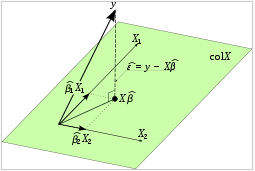
\includegraphics[height=2in]{OLS}}

\end{frame}

\begin{frame}
  \frametitle{Properties}
 $\Yhat = \muhat$ is an unbiased estimate of $\mub = \X\b$
\pause
    \begin{eqnarray*}
      \E [ \Yhat ]  & = & \E [\P_\X \Y ] \pause\\
& = & \P_\X \E[\Y] \pause\\
& = & \P_\X \mub \pause\\
& = & \mub \pause
    \end{eqnarray*}

$\E[\e] = \zero$ if $\mub \in C(\X)$ \pause
\begin{eqnarray*}
      \E [ \e ]  & = & \E [(\I - \P_\X) \Y ] \pause\\
& = & (\I - \P_\X) \E[\Y] \pause\\
& = & (\I - \P_\X) \mub \pause\\
& = & \zero \pause
    \end{eqnarray*}
Will not be $\zero$ if $\mub \notin C(\X)$  (useful for model checking)

\end{frame}

\begin{frame}
  \frametitle{Estimate of $\sigma^2$}
MLE of $\sigma^2$:
  $$\shat = \frac{\e^T\e}{n} = \frac{\Y^T (\I - \P_\X) \Y}{n}$$
\pause
Is this an unbiased estimate of $\sigma^2$?
\pause

\vspace{1in}
Need expectations  of quadratic forms $\Y^T \A \Y$ for $\A$ an
 $n \times n$ matrix $\Y$ a random vector in $\bbR^n$
\end{frame}
\begin{frame}
  \frametitle{Quadratic Forms}
  Without loss of generality we can assume that $\A = \A^T$
\pause
  \begin{itemize}
  \item $\Y^T \A \Y$ is a scalar \pause
\item $\Y^T \A \Y  = (\Y ^T\A  \Y)^T = \Y^T \A^T \Y$ \pause
  \begin{eqnarray*}
 \frac{\Y^T \A \Y  + \Y^T \A^T \Y}{2} & = &
\Y^T \A \Y  \pause \\
    \Y^T\frac{(\A + \A^T)}{2}\Y  & = & \Y^T \A \Y \pause
  \end{eqnarray*}
\item may take $\A = \A^T$
  \end{itemize}
\end{frame}
\begin{frame}
  \frametitle{Expectations of Quadratic Forms}
  \begin{theorem}
   Let  $\Y$ be a random vector in $\bbR^n$ with $\E[\Y] = \mub$ and
   $\Cov(\Y) = \Sigmab$.  \pause Then $\E[\Y^T \A \Y] = \tr \A \Sigma + \mub^T
   \A \mub$.
  \end{theorem} \pause
Result useful for finding expected values of Mean Squares; no
normality required!
\end{frame}
\begin{frame}
  \frametitle{Proof}
Start with $(\Y - \mub)^T\A (\Y - \mub)$,  expand and take
expectations \pause
  \begin{eqnarray*}
\E [(\Y - \mub)^T\A (\Y - \mub)] & = & \E[\Y^T\A \Y + \mub^T\A \mub -
    \mu^T\A \Y - \Y^T \A \mu] \pause \\
 & = & \E[\Y^T\A \Y] + \mub^T\A \mub -
\mub^T\A \mub - \mub^T\A \mub \pause \\
 & = & \E[\Y^T\A \Y] - \mub^T\A \mub \pause 
  \end{eqnarray*}
Rearrange \pause
 \begin{eqnarray*}
 \E[\Y^T\A \Y ] & = &  \E[ (\Y - \mub)^T\A (\Y - \mub)] + \mub^T\A
 \mub \pause \\
 & = & \E[ \tr (\Y - \mub)^T\A (\Y - \mub)] + \mub^T\A \mub  \pause\\
 & = & \E[ \tr \A (\Y - \mub) (\Y - \mub)^T] + \mub^T\A
 \mub \pause \\
 & = &\tr  \E[ \A (\Y - \mub) (\Y - \mub)^T] + \mub^T\A \mub \pause \\
 & = &\tr \A \E([ (\Y - \mub) (\Y - \mub)^T] + \mub^T\A \mub \pause \\
 & = &\tr \A \Sigmab + \mub^T\A \mub  \pause
\end{eqnarray*}
\alert<12>{{\small{$\tr \A \equiv \sum_{i=1}^n a_{ii}$}}}
\end{frame}
\begin{frame}
  \frametitle{Expectation of $\shat$}
  
Use the theorem: \pause
\begin{eqnarray*}
\E[\Y^T (\I - \P_\X) \Y] & = &\tr (\I - \P_\X) \sigma^2 \I +
\mub^T(\I - \P_\X) \mub  \pause \\
 & = &  \sigma^2 \tr (\I - \P_\X) \pause \\
 & = & \sigma^2 r(\I - \P_\X) \pause\\
& = & \sigma^2 (n - r(\X)) \pause
\end{eqnarray*}


Therefore an unbiased estimate of $\sigma^2$ is $$\frac{\e^T\e}{n - r(\X)}$$
\pause

If $\X$ is full rank ($r(\X) = p$) and $\P_{\X} = \X(\X^T\X)^{-1} \X^T$ then the 

\begin{eqnarray*}
\tr(\P_{\X}) & = & \tr( \X(\X^T\X)^{-1} \X^T) \\
&  = &  \tr(\X^T\X(\X^T\X)^{-1}) \\
&  = & \tr(\I_p) = p
\end{eqnarray*}


\end{frame}
\begin{frame}
  \frametitle{Spectral Theorem}
  \begin{theorem}
    If $\A$ ($n \times n$) is a symmetric real matrix  then there
    exists a  $\U$ ($n \times n$) such that $\U^T\U = \U \U^T = \I_n$
     and a diagonal matrix $\Lambdab$ with
    elements $\lambda_i$ such that $\A = \U \Lambdab \U^T$
  \end{theorem} \pause
  \begin{itemize}
  \item $\U$ is an orthogonal matrix; $\U^{-1} = \U^T$ \pause
  \item The columns of $\U$ from an Orthonormal Basis for $\bbR^n$ \pause
  \item rank of $\A$ equals the number of non-zero eigenvalues
    $\lambda_i$ \pause
  \item Columns of $\U$ associated with non-zero eigenvalues form an
    ONB for $C(\A)$ (eigenvectors of $\A$) \pause
\item $\A^p = \U \Lambdab^p \U^T$ (matrix powers) \pause
\item a square root of $\A > 0$ is $\U \Lambdab^{1/2}\U^T$ \pause
  \end{itemize}
\end{frame}
\begin{frame}
  \frametitle{Projections}
\begin{block}{Projection Matrix}
If $\P$ is an orthogonal projection matrix, then its eigenvalues
$\lambda_i$ are
either zero or one with $\tr (\P) = \sum_i(\lambda_i) = r(\P)$
\end{block} \pause
\begin{itemize}
\item   $\P = \U \Lambdab \U^T $  \pause
\item $\P = \P^2$  $\Rightarrow$ $\U \Lambdab \U^T\U \Lambdab \U^T =
  \U\Lambdab^2\U^T$  \pause
\item $\Lambdab = \Lambdab^2$ is true only for $\lambda_i = 1$ or
  $\lambda_i =0$  \pause
\item Since $r(\P)$ is the number of non-zero eigenvalues, $r(\P) =
  \sum \lambda_i = \tr(\P)$  \pause
\end{itemize}
$$\P = \left[\U_P \U_{P^\perp} \right] 
\left[
  \begin{array}{ll}
    \I_r & \zero \\
    \zero & \zero_{n-r}
  \end{array}
\right] \left[
  \begin{array}{l}
    \U_P^T \\
\U^T_{P^\perp}
  \end{array}
\right] = \U_P \U^T_P$$
$$\P = \sum_{i=1}^r \u_i \u_i^T$$  
sum of $r$ rank 1 projections.
\end{frame}


\section{Multivariate Normal}

\begin{frame} \frametitle{Distributions}
  \begin{itemize}
  \item Distribution of $\hat{\b}$
  \item Distribution of $\P_{\X} \Y$
  \item Distribution of $\e$
  \item Distribution ot $\hat{\sigma^2}$
  \end{itemize}
\end{frame}
\begin{frame}
  \frametitle{Univariate Normal}

  \begin{definition}
  We say that $Z$ has a standard  Normal distribution  
$$Z \sim  \N(0,1)$$ with mean 0 and variance 1 if it has density \pause
$$
f_Z(z) = \frac{1}{\sqrt{2 \pi}} e^{-\frac 1 2 z^2}
$$
  \end{definition} \pause

If $Y = \mu + \sigma  Z$ then $Y \sim N(\mu, \sigma^2)$ 
with mean $\mu$ and variance $\sigma^2$  \pause
$$
f_Y(y) = \frac{1}{\sqrt{2 \pi \sigma^2}} e^{-\frac 1 2 \left(\frac{z - \mu}{\sigma}\right)^2}
$$
  
\end{frame}

\begin{frame}
  \frametitle{Standard Multivariate Normal}
Let  $z_i \simiid \N(0, 1)$ for $i = 1, \ldots, d$ and  define
 $$\Z \equiv \left[
  \begin{array}{c}
    z_1 \\ z_2 \\ \vdots \\ z_d 
  \end{array}
\right]
$$ \pause


 \begin{itemize}
 \item Density of $Z$: \pause
\begin{eqnarray*}
f_{\Z}(\z) & = \prod_{j=1}^d \frac{1}{ \sqrt{2 \pi}} e^{-z_i^2/2}  \pause \\
 \, & = (2\pi)^{-d/2}e^{- \frac{1}{2} (\Z^T\Z)} \pause
\end{eqnarray*}
\item $\E[\Z] = \zero$ and $\Cov[\Z] =  \I_d$   \pause
\item $\Z \sim \N(\zero_d, \I_d)$ \pause

\end{itemize}
\end{frame}

\frame{ \frametitle{Multivariate Normal}

  For a $d$ dimensional multivariate normal random vector, we write
  $\Y \sim N_d(\mub, \Sigmab)$ \pause

  \begin{itemize}
  \item<2-> $\E[\Y] = \mub$:  $d$ dimensional vector with means
    $E[Y_j]$ \pause
  \item<3-> $\Cov[\Y] = \Sigmab$: $d \times d$ matrix with diagonal elements
    that are the variances of $Y_j$ and off diagonal elements that are
    the covariances $\E[(Y_j - \mu_j)(Y_k - \mu_k)]$ \pause
  \end{itemize}
 \only<4>{ \begin{block}{Density}
 If $\Sigmab$ is positive definite ($\x'\Sigmab \x > 0$ for any $\x \ne
  0$ in $\bbR^d$) then $\Y$ has  a density \footnote{ with respect to Lebesgue
  measure on $\bbR^d$} \pause

$$p(\Y) = (2 \pi)^{-d/2} |\Sigmab|^{-1/2} \exp(-\frac{1}{2}(\Y - \mub)^T
\Sigmab^{-1} (\Y - \mub))$$    
  \end{block}}
}
\frame{ \frametitle{Multivariate Normal Density}
\begin{itemize}
 \item<1-> Density of $Z \sim \N(\zero, \I_d)$:
\begin{eqnarray*}
\onslide<2->{f_{\Z}(\z) & = \prod_{j=1}^d \frac{1}{ \sqrt{2 \pi}} e^{-z_i^2/2} } \\
\onslide<3->{ \, & = (2\pi)^{-d/2}e^{- \frac{1}{2} (\Z^T\Z)}}
\end{eqnarray*}
\item<4->  Write $\Y = \mub + \A \Z$  
\item<5-> Solve for $\Z = g(\Y)$ 
\item<6-> Jacobian of the
  transformation  $J(\Z \rightarrow \Y) = | \frac{\partial
    g}{\partial \Y} |$ 
\item<7>substitute  $g(\Y)$ for $\Z$ in density and
  multiply by Jacobian
{$$  f_\Y(\y)  = f_\Z(\z) J(\Z \rightarrow \Y) $$}
\end{itemize}
}
\frame{ \frametitle{Multivariate Normal Density}
   \begin{equation} \Y  = \mub + \A \Z   \quad    \text{ for }  \Z \sim \N(\zero, \I_d) \end{equation}

  \begin{proof}
  \begin{itemize}
   \item<2->  since  $\Sigmab > 0, \, \exists$
   an $\A$ ($d \times d$) such that $\A > 0$ and $\A
  \A^T = \Sigmab$ 
\item<3-> { $\A >0  \Rightarrow   \A^{-1}$ exists}
\item<4-> Multiply both sides (1)  by $\A^{-1}$: $$\alert<4>{\A^{-1}}\Y =
  \alert<4>{\A^{-1}} \mub + \alert<4>{\A^{-1}}\A \Z$$
\item<5-> Rearrange $\A^{-1} (\Y - \mub) = \Z $ 
\item<6-> Jacobian of transformation $d\Z = |\A^{-1}| d\Y$
\item<7->  Substitute and simplify  algebra
  \end{itemize}
\onslide<7>{$$f(\Y) = (2 \pi)^{-d/2} |\Sigmab|^{-1/2} \exp(-\frac{1}{2}(\Y - \mub)^T
\Sigmab^{-1} (\Y - \mub))$$  }
  \end{proof}
  
}

\begin{frame} \frametitle{Singular Case}
$\Y = \mub + \A \Z$  with $\Z \in \bbR^d$ and $\A$ is $n \times d$ \pause
\begin{itemize}
\item $\E[\Y] = \mu$ \pause
\item $\Cov(\Y) = \A \A^T \ge 0$ \pause
\item $\Y \sim \N(\mub, \Sigmab)$ where $\Sigmab = \A \A^T$
\end{itemize}
  If $\Sigmab$ is singular then there is no density (on $\bbR^n$), but claim that
  $\Y$ still has a multivariate normal distribution!  \pause

 \begin{definition}
  $\Y \in \bbR^n$ has a  multivariate normal distribution $\N(\mub,
  \Sigmab)$ if for any $\v \in \bbR^n$ $\v^T\Y$ has a normal
  distribution with mean $\v^T\mub$ and variance $\v^T\Sigmab \v$
  \end{definition} \pause

see
\href{https://sakai.duke.edu/portal/site/79ac6ecf-19ee-496f-889b-1b3f6668eca9/page/3ea2b213-a451-4743-a788-610173b5b888}{Lessons
  in Sakai for videos using Characteristic functions}
\end{frame}

\begin{frame} \frametitle{Linear Transformations are Normal}

If $\Y \sim \N_n(\mub, \Sigmab)$ then for $\A$ $m \times n$

$$\A \Y \sim \N_m(\A \mub, \A \Sigmab \A^T)$$


$\A \Sigmab \A^T$ does not have to be positive definite!
  


\end{frame}
\begin{frame}
  \frametitle{Equal in Distribution}
  Multiple ways to define the same normal: \pause

  \begin{itemize}
  \item 
$\Z_1 \sim \N(\zero, \I_n)$, $\Z_1 \in \bbR^n$  and take $\A$ $d
\times n$ \pause
\item $\Z_2 \sim \N(\zero, \I_p)$,  $\Z_2 \in \bbR^p$  and take $\B$ $d
\times p$ \pause
\item Define $\Y = \mub + \A \Z_1$ \pause
\item Define $\W = \mub + \B \Z_2$ \pause
  \end{itemize}
  \begin{theorem}
    If  $\Y = \mub + \A \Z_1$ and $\W = \mub + \B \Z_2$ then $\Y
    \eqindis \W$ if and only if $\A \A^T = \B \B^T = \Sigmab$
  \end{theorem}
\end{frame}

\frame{ \frametitle{Zero Correlation and Independence}
 \begin{theorem}
For a random vector $\Y \sim \N(\mub, \Sigmab) $ partitioned as
$$
\Y = \left[
  \begin{array}{c}
\Y_1  \\ \Y_2 \end{array} \right]  \sim \N\left( \left[
  \begin{array}{c} \mub_1  \\ \mub_2 \end{array} \right],
  \left[ \begin{array}{cc}
\Sigmab_{11} &  \Sigmab_{12}  \\ 
\Sigmab_{21} & \Sigmab_{22} \end{array} \right]
 \right)    
 $$  \pause
then $\Cov(\Y_1, \Y_2) = \Sigmab_{12} = \Sigmab_{21}^T = \zero$  if and
only if $\Y_1$ and $\Y_2$ are independent.
  \end{theorem}
}

\frame { \frametitle{Independence Implies Zero Covariance}
\begin{proof}
$$ \Cov(\Y_1, \Y_2) = \E[ (\Y_1 - \mub_1)(\Y_2 - \mub_2)^T]$$ \pause
  If $\Y_1$ and $\Y_2$ are independent \pause 
$$\E[ (\Y_1 - \mub_1)(\Y_2 - \mub_2)^T] = \E[ (\Y_1 - \mub_1) \E(\Y_2 -
\mub_2)^T] = \zero \zero^T = \zero $$ \pause
 
therefore $\Sigmab_{12} = \zero$

\end{proof}

}

\frame { \frametitle{ Zero Covariance Implies  Independence}
  Assume $\Sigmab_{12} = \zero$
\begin{block}{Proof}
\begin{itemize}

\item  Choose an $$ 
  \A = \left[
  \begin{array}{ll}
    \A_1 & \zero \\
    \zero & \A_2 
  \end{array}
\right]  $$
 such that $\A_1 \A_1^T = \Sigmab_{11}$, $\A_2 \A_2^T = \Sigmab_{22}$
 \pause
 \item Partition  $$
\Z = \left[
  \begin{array}{c}
    \Z_1 \\ \Z_2
  \end{array}
\right] \sim \N\left(
\left[
  \begin{array}{c}
    \zero_1 \\ \zero_2
  \end{array}
\right],
\left[
  \begin{array}{ll}
    \I_1 &\zero \\
\zero & \I_2
  \end{array}
\right]  
 \right)  \text{ and } \mub = \left[
  \begin{array}{c}
    \mub_1 \\ \mub_2
  \end{array}
\right] $$ \pause
\item then 
       $\Y \eqindis \A \Z + \mub \sim  \N(\mub, \Sigmab)$ 
\end{itemize}
  \end{block}  
}
\frame {\frametitle{Continued}
  \begin{proof}
    \begin{itemize}
    \item $$
\left[
  \begin{array}{c}
    \Y_1 \\ \Y_2
  \end{array}
\right]  \eqindis \left[
  \begin{array}{c}
    \A_1\Z_1 + \mub_1 \\ \A_2\Z_2 +\mub_2
  \end{array}
\right] 
$$ \pause
\item But $\Z_1$ and $\Z_2$ are independent \pause
\item Functions of $\Z_1$ and $\Z_2$ are independent \pause
\item Therefore $\Y_1$ and $\Y_2$ are independent  \pause
    \end{itemize}
  \end{proof}
For Multivariate Normal Zero Covariance implies independence

}
\frame { \frametitle{ Another Useful Result}
  \begin{corollary}
    If $\Y \sim \N( \mub, \sigma^2 \I_n) $ and $\A \B^T = \zero$
then $\A \Y$ and $\B \Y$ are independent.
  \end{corollary} \pause
  \begin{proof}
 \begin{itemize}
    \item $$
\left[
  \begin{array}{c}
    \W_1 \\ \W_2
  \end{array}
\right]  = \left[
  \begin{array}{c}
    \A \\ \B 
  \end{array}
\right]  \Y =  \left[
  \begin{array}{c}
    \A \Y \\ \B  \Y
  \end{array}
\right] 
$$ \pause
\item $\Cov(\W_1, \W_2) = \Cov(\A \Y, \B \Y) = \sigma^2 \A \B^T$
  \pause
\item $\A \Y $ and $\B \Y$ are independent if $\A \B^T = \zero$
\end{itemize}    
  \end{proof}

}

\end{document}
\frame{ \frametitle{Conditional Distributions}

  \begin{Theorem}
If    $$
\Y = \left[
  \begin{array}{c}
\Y_1  \\ \Y_2 \end{array} \right]  \sim \N\left( \left[
  \begin{array}{c} \mub_1  \\ \mub_2 \end{array} \right],
  \left[ \begin{array}{cc}
\Sigmab_{11} &  \Sigmab_{12}  \\ 
\Sigmab_{21} & \Sigmab_{22} \end{array} \right]
 \right)    
 $$
 and $\Sigma_{22} > 0$
then
$$\Y_1 \mid \Y_2 = \y_2 \sim \N\left( \mub_1 + \Sigmab_{12}
\Sigmab_{22}^{-1} (\y_2 - \mub_2), \Sigmab_{11} - \Sigmab_{12}
\Sigmab_{22}^{-1} \Sigmab_{21}\right)$$
 \end{Theorem}\pause

 \begin{itemize}
 \item 
The conditional distribution of $\Y_1$ given $\Y_2$ is also normal!
\pause

\item Can replace $\Sigmab_{22}^{-1}$ by a Generalized inverse if
$\Sigmab_{22}$ is singular.
 \end{itemize}

}

\begin{frame}
  \frametitle{Derivation}
  \begin{block}{Proof}
    \begin{itemize}
    \item Define
$$  \left[
  \begin{array}{c} 
\W_1  \\ \W_2 \end{array} \right] =  \left[ \begin{array}{cc}
\I & -\Sigmab_{12} \Sigmab_{22}^{-1}  \\ \zero & \I \end{array} \right]  \left[
  \begin{array}{c}
\Y_1  \\ \Y_2 \end{array} \right] =  \left[
  \begin{array}{c}
\Y_1 - \Sigmab_{12} \Sigmab_{22}^{-1} \Y_2  \\ \Y_2 \end{array} \right]
 $$ 
\pause
\item  then
$$\W_1 \sim \N\left( \mub_1 - \Sigmab_{12} \Sigmab_{22}^{-1} \mub_2,
\Sigmab_{11} - \Sigmab_{12}\Sigmab_{22}^{-1} \Sigmab_{21} \right) $$ \pause
$$\W_2 \sim \N(\mub_2, \Sigmab_{22})$$ \pause
$$\Cov(\W_1, \W_2) = \zero$$
  \end{itemize}
  \end{block}
\end{frame}
\begin{frame}
  \frametitle{Covariance of $\W_1$ and $\W_2$}
  \begin{block}{}
    
    $$\Cov(\W_1, \W_2) = \left[\I \, -\Sigmab_{12}
        \Sigmab_{22}^{-1} \right]   \left[ \begin{array}{cc}
\Sigmab_{11} &  \Sigmab_{12}  \\ 
\Sigmab_{21} & \Sigmab_{22} \end{array} \right] \left[  
\begin{array}{c} \zero \\ \I \end{array}
\right] $$
  \end{block}
\end{frame}
\begin{frame}
  \frametitle{Conditional Characteristic Function }
  \begin{block}{} 
    \begin{itemize}
    \item 
    $\varphi_{\Y_1 \mid \Y_2 = \y_2}(t) = \E \left[ e^{i t^T \Y_1} \mid \Y_2 =
      \y_2 \right]$ \pause
\item Add zero
$$
 = \E \left[ e^{i t^T \Y_1  \alert<2>{-i t^T \Sigmab_{12}\Sigmab_{22}^{-1} \Y_2 +
     i t^T \Sigmab_{12}\Sigmab_{22}^{-1} \Y_2 } } \mid \Y_2 =
      \y_2 \right]
$$  \pause
\item Factor and exploit conditioning 
  \begin{eqnarray*}
&  = \E \left[ e^{i t^T \alert<4>{\Y_1  -i t^T \Sigmab_{12}\Sigmab_{22}^{-1} \Y_2}}
      \,  e^{
     i t^T \Sigmab_{12}\Sigmab_{22}^{-1} \Y_2 }  \mid \Y_2 =
      \y_2 \right]  \pause
\\
&  = \E \left[ e^{i t^T \W_1} \mid \Y_2 = \y_2 \right] \alert<4>{e^{
     i t^T \Sigmab_{12}\Sigmab_{22}^{-1} \y_2 }}     
  \end{eqnarray*} \pause
\item Independence of
   $\W_1 = \Y_1 - \Sigma_{12}\Sigma_{22}^{-1}$ and $\Y_2 = \W_2$
$$ = \E \left[ e^{i t^T \W_1} \right]\,  e^{
     i t^T \Sigmab_{12}\Sigmab_{22}^{-1} \y_2 }  $$ 
   \end{itemize}

  \end{block}
\end{frame}
\begin{frame}
  \frametitle{Combine}
  \begin{block}{}
    \begin{itemize}
    \item $\W_1 \sim \N( \mub_1 - \Sigmab_{12} \Sigmab_{22}^{-1}
      \mub_2, \Sigmab_{11} - \Sigmab_{12} \Sigmab_{22}^{-1}
      \Sigmab_{21})$ \pause
$$\varphi_{\W_1}(t) = e^{i t^T( \mub_1 - \Sigmab_{12} \Sigmab_{22}^{-1}
      \mub_2) - \frac{1}{2} t^T (\Sigmab_{11} - \Sigmab_{12} \Sigmab_{22}^{-1}
      \Sigmab_{21})t}$$ \pause
\item Combining
  \begin{eqnarray*}
\varphi_{\Y_1 \mid \Y_2} (t)  =  & \varphi_{\W_1}(t) \, e^{  i t^T
    \Sigmab_{12}\Sigmab_{22}^{-1} \y_2 } \pause \\ 
    = & e^{i t^T( \mub_1 - \Sigmab_{12} \Sigmab_{22}^{-1}
      \mub_2) - \frac{1}{2} t^T (\Sigmab_{11} - \Sigmab_{12} \Sigmab_{22}^{-1}
      \Sigmab_{21})t} \, e^{  i t^T
    \Sigmab_{12}\Sigmab_{22}^{-1} \y_2 } \pause   \\   
 =  & e^{i t^T( \mub_1 + \Sigmab_{12} \Sigmab_{22}^{-1}( \y_2 -
      \mub_2) - \frac{1}{2} t^T (\Sigmab_{11} - \Sigmab_{12} \Sigmab_{22}^{-1}
      \Sigmab_{21})t} 
  \end{eqnarray*} \pause
\item Characteristic function implies
$$
\Y_1 \mid \Y_2 \sim \N( \mub_1 + \Sigmab_{12} \Sigmab_{22}^{-1}( \y_2 -
      \mub_2),  \Sigmab_{11} - \Sigmab_{12} \Sigmab_{22}^{-1}
      \Sigmab_{21})
$$ 
  \end{itemize}
  \end{block}
\end{frame}

\begin{frame}
  \frametitle{Regression setting}
  Let $\Y_1 = Y$ and  $\Y_2 = \x$   

Then 
$$
Y \mid \X \sim \N( \mub_1 + \Sigmab_{12} \Sigmab_{22}^{-1}( \x -
      \mub_2),  \Sigmab_{11} - \Sigmab_{12} \Sigmab_{22}^{-1}
      \Sigmab_{21})
$$ 

$$
Y \mid \X \sim \N( \mub_1 - \Sigmab_{12} \Sigmab_{22}^{-1} \mu_2  + \Sigmab_{12} \Sigmab_{22}^{-1} \x ,  \Sigmab_{11} - \Sigmab_{12} \Sigmab_{22}^{-1}
      \Sigmab_{21})
$$ 

$$
Y_i \mid \X \sim \N( \beta_0  + \x_i^T \b ,  \sigma^2)
$$

Multivariate Normality is not necessary 
\end{frame}

\begin{frame}
  \frametitle{General Definition }
  \begin{definition}
  Let $\V$ be an vector  space with inner product $\langle ,
  \rangle$.  Then
  $\Y \in \V$ has a  multivariate normal distribution $\N(\mub,
  \Sigmab)$ if for any $\v \in \V$, $\langle \v, \Y \rangle$ has a normal
  distribution with mean $\langle \v,\mub \rangle $ and variance
  $\langle \v,  \Sigmab \v \rangle$
  \end{definition} \pause

For usual Euclidean space inner product $\langle \x, \y \rangle =
\x^T\y$ \pause

\vfill
For the energetic Student:  Consider space of $n \times m$ matrices,
and a random matrix $\Y \sim \N(\mub, \I \otimes \Sigmab)$
where  $(\I \otimes \Sigmab) M = \I M \Sigmab^T$ for $M$ $n \times m$
\pause
\vfill
Under the Inner product $\langle \x, \y \rangle \equiv \tr \x \y$, show that $
\Y$ has a multivariate normal distribution on the space of $n \times
m$  matrices
\end{frame}

\end{document}